\documentclass[11pt,a4paper]{article}

\usepackage[margin=2.3cm]{geometry}
\usepackage[T1]{fontenc}
\usepackage{lmodern}
\usepackage{microtype}
\usepackage{graphicx}
\usepackage{booktabs}
\usepackage{xcolor}
\usepackage{tikz}
\usetikzlibrary{arrows.meta,positioning}
\usepackage{caption}
\usepackage{enumitem}
\usepackage{amsmath}
\usepackage[hidelinks]{hyperref}
\usepackage{float}

\setlist{itemsep=2pt,topsep=4pt}
\captionsetup{font=small,labelfont=bf}
\definecolor{boxblue}{HTML}{E8F1FC}
\definecolor{boxline}{HTML}{2A78D6}
\definecolor{boxgreen}{HTML}{E7F6EF}
\definecolor{linegreen}{HTML}{1BAF7A}

\newcommand{\pRows}{12,950}
\newcommand{\pPos}{3,143}
\newcommand{\pNeg}{9,807}
\newcommand{\pGold}{3,580}
\newcommand{\pPseudo}{9,188}
\newcommand{\pAudited}{182}
\newcommand{\pDupDropped}{1,553}
\newcommand{\pPrefevalTurns}{8,757}
\newcommand{\pOasstPool}{15,427}
\newcommand{\pOasstRev}{fdf72ae0}
\newcommand{\pPersonaFound}{998}
\newcommand{\pOverlapAgree}{95.3}
\newcommand{\pOasstYes}{289}
\newcommand{\pStrictConfirmed}{115}
\newcommand{\pStrictRejected}{174}
\newcommand{\pGenericExcl}{1,384}
\newcommand{\pStrictExcl}{791}
\newcommand{\pGenericPrec}{0.28}
\newcommand{\pStrictPrec}{0.60}
\newcommand{\pAuditBefore}{73.9}
\newcommand{\pAuditAfter}{90.7}
\newcommand{\pKappa}{0.48}
\newcommand{\pTopicRateLo}{0.35}
\newcommand{\pTopicRateHi}{0.41}
\newcommand{\pFOneLo}{0.969}
\newcommand{\pFOneHi}{0.976}
\newcommand{\pBestEnsFOne}{0.977}
\newcommand{\pBestEnsMembers}{TinyLlama + Qwen3}
\newcommand{\pErrCorrLo}{0.68}
\newcommand{\pErrCorrHi}{0.75}
\newcommand{\pDisagreeMax}{0.9}
\newcommand{\pLlmFOne}{0.879}
\newcommand{\pLlmPrec}{0.787}
\newcommand{\pLlmRec}{0.996}
\newcommand{\pLlmFpr}{16.5}
\newcommand{\pLlmLat}{72}
\newcommand{\pDistilLat}{1.4}
\newcommand{\pSpeedup}{51}
\newcommand{\pDistilSameFOne}{0.990}
\newcommand{\pOodLo}{0.1}
\newcommand{\pOodHi}{1.5}
\newcommand{\pTotalTrainH}{4.3}
\newcommand{\pOasstRecLo}{16}
\newcommand{\pOasstRecHi}{26}
\newcommand{\pOasstPosTest}{114}

\graphicspath{{../results/phase2/figures/}}

\title{\textbf{Improving Long-Context Preference Following in LLMs}\\[2pt]
\large Phase 2 Report: A Trained Preference-Detection Classifier}
\author{Krishna Jhanwar (12341250)\\ \small\texttt{krishnaj@iitbhilai.ac.in}}
\date{October 2026}

\begin{document}
\maketitle

\begin{abstract}
\noindent
Phase~2 trains a small classifier that answers one question about every user message: \emph{does it state a preference?}
In Phase~3 this classifier decides which turns enter a structured preference memory. I built a turn-level dataset of
\pRows{} messages from PrefEval and OpenAssistant. It combines \pGold{} labels taken from the dataset's structure, \pPseudo{}
labels produced by a local LLM, and \pAudited{} human-audited labels. A 200-row manual audit exposed systematic pseudo-label errors;
targeted refinement raised agreement with the human labels from \pAuditBefore\% to \pAuditAfter\%. Four models (DistilBERT, ModernBERT,
TinyLlama-1.1B and Qwen3-1.7B, the last two with LoRA) were trained with topic-level 5-fold cross-validation, so every test
topic is unseen. All four reach F1 \pFOneLo--\pFOneHi{} and are statistically close. Their errors are highly correlated, so the best of 15
ensembles adds only $+0.001$ F1. Against a prompted Llama-3-8B on the same 2{,}000 messages, the classifiers score F1 0.990--0.994 versus
\pLlmFOne, and DistilBERT is about \pSpeedup$\times$ faster (\pDistilLat\,ms vs.\ \pLlmLat\,ms per message). The models raise almost no
false alarms on real chat (\pOodLo--\pOodHi\%) but miss most casual real-chat preferences, which is the main limitation.
\end{abstract}

%===============================================================================
\section{Role in the project}
PrefEval shows that LLMs lose track of user preferences as a conversation grows (Phase~1 reproduced this locally). The proposal's
answer is a structured \emph{preference memory}: every incoming user turn is checked by a cheap classifier, and turns that state
a preference are stored and re-inserted near the question. Phase~2 builds that classifier and tests the proposal's claim that one small
forward pass can replace LLM-prompted preference detection.

%===============================================================================
\section{Task definition}
\begin{itemize}
  \item \textbf{Unit and input.} One user message. The model's \emph{only} input is the raw text of that message: no conversation
        history, no assistant turns, no topic or other metadata. It is truncated to 256 tokens; all PrefEval messages are $\le$130 tokens.
        This matches Phase~3, where the classifier sees each turn as it arrives.
  \item \textbf{Output.} $p = P(\text{preference} \mid \text{text})$. The decision is $p \ge \tau$, with the threshold $\tau$ tuned on each fold's
        \emph{validation} split to maximise F1.
  \item \textbf{Label 1:} the message reveals a lasting personal preference, dislike, restriction or constraint of the user that should
        shape future recommendations, whether stated directly or implied by a choice or a passing remark. \textbf{Label 0:} plain
        requests, questions, task requirements (``use Python 3.7''), feedback on the current output, small talk, statements about other people.
\end{itemize}

%===============================================================================
\section{Data}

\subsection{Sources and labels}
Table~\ref{tab:data} lists every source. PrefEval provides three kinds of \emph{gold} labels through its structure:
explicit preference sentences are positives; choice-based dialogues contain one selection turn that reveals a preference (positive);
and the initial queries and final questions contain none (negatives). Exact-duplicate texts were removed (\pDupDropped{} dropped).
Two sources have no labels and were \emph{pseudo-labelled} once, offline, by Llama-3-8B-Instruct (Ollama, temperature 0):

\begin{itemize}
  \item \textbf{Persona dialogues.} Each persona dialogue hides its known preference in one user turn, but the dataset does not mark which.
        For each dialogue the LLM was given the reference preference and the numbered user turns, and asked which turn reveals it
        (found in \pPersonaFound{} of 1{,}000 dialogues). An independent, LLM-free word-overlap check agreed in \pOverlapAgree\% of cases.
        The authors placed the preference in user turn~2 in about 66\% of dialogues; the classifier never sees turn positions, so this
        pattern cannot become a shortcut.
  \item \textbf{OpenAssistant.} 5{,}000 English user messages were sampled with a fixed seed from \pOasstPool{} in \texttt{oasst1}
        (dataset revision \texttt{\pOasstRev}), to add realistic chat that is mostly preference-free. The LLM labelled each one YES or NO.
\end{itemize}

\begin{table}[H]
\centering\small
\begin{tabular}{llrrr}
\toprule
Source & Label origin & Label 1 & Label 0 & Rows \\
\midrule
Explicit preference & gold & 988 & 0 & 988 \\
Persona preference field & gold & 30 & 0 & 30 \\
Choice selection (implicit) & gold & 991 & 0 & 991 \\
Persona dialogue turn & pseudo (LLM) & 1,020 & 3,355 & 4,375 \\
Choice initial query & gold & 0 & 577 & 577 \\
Final question & gold & 0 & 994 & 994 \\
OpenAssistant message & pseudo (LLM) & 114 & 4,881 & 4,995 \\
\midrule Total & & 3,143 & 9,807 & 12,950 \\
\bottomrule
\end{tabular}

\caption{Final training data after refinement and audit overrides. Persona-turn and OpenAssistant labels are refined LLM pseudo-labels;
182 rows carry the human audit label.}
\label{tab:data}
\end{table}

\subsection{Manual audit and label refinement}
A stratified sample of 200 pseudo-labelled rows (40 per stratum) was labelled by hand, following written guidelines. The
audit found two systematic error types (Table~\ref{tab:audit}):
\begin{enumerate}
  \item \textbf{OpenAssistant ``yes'' labels were only 40\% correct.} The LLM treated task requirements and one-off requests as
        preferences. All \pOasstYes{} YES rows were re-checked with a stricter prompt (``a \emph{lasting personal} preference of the
        user''). \pStrictConfirmed{} were confirmed, and the \pStrictRejected{} rejected rows became \emph{hard negatives}.
  \item \textbf{Persona labels missed preferences stated twice.} When the LLM and the overlap check picked different turns, the
        overlap turn also revealed the preference in every disagreement error. Positives are therefore the \emph{union} of both picks
        (overlap only with $\ge$2 shared content words). Other turns that still state a preference were filtered out as ambiguous. Two filters
        were compared against the audit: a generic prompt excluded \pGenericExcl{} turns with flag precision \pGenericPrec; a strict prompt
        excluded \pStrictExcl{} with precision \pStrictPrec{}. The strict filter was kept.
\end{enumerate}

\begin{table}[H]
\centering\small
\begin{tabular}{lrrr}
\toprule
Audit stratum & $n$ & Before refinement & After refinement \\
\midrule
Persona, LLM-picked turn (+) & 40 & 1.000 & 1.000 \\
Persona, other turns (-) & 39 & 0.821 & 0.966 \\
Persona, LLM vs overlap disagree & 40 & 0.475 & 0.909 \\
OpenAssistant, LLM yes (+) & 40 & 0.400 & 0.675 \\
OpenAssistant, LLM no (-) & 40 & 1.000 & 1.000 \\
\midrule All strata & 199 & 0.739 ($\kappa$=0.48) & 0.907 \\
\bottomrule
\end{tabular}

\caption{Agreement between pseudo-labels and the human audit, before and after refinement. ``After'' is measured on the same
audited rows that motivated the fixes, so it is somewhat optimistic. The audited rows themselves use the human label in training.}
\label{tab:audit}
\end{table}

\subsection{Splits and leakage control}
\begin{itemize}
  \item \textbf{Topic-level 5-fold cross-validation.} PrefEval's 20 topics are shuffled into 5 folds of 4. In round $k$: test = fold $k$,
        validation = fold $k{+}1$, train = the remaining 3. PrefEval contains many near-identical sentences within a topic, so a random split would
        inflate scores; testing on unseen topics measures generalisation. OpenAssistant rows are assigned by conversation tree.
  \item \textbf{LMSYS distractor turns are never trained on.} Phase~3 replays the same 316 LMSYS turns in every evaluation question, so
        they serve only as an out-of-domain (OOD) test of false alarms.
  \item Both rules are asserted in code. Per-topic positive rates lie between \pTopicRateLo{} and \pTopicRateHi, so topic identity
        does not predict the label.
\end{itemize}

%===============================================================================
\section{Models and training}

\begin{center}\small
\begin{tabular}{llllr}
\toprule
Model & Type & Fine-tuning & Precision & LR, epochs \\
\midrule
DistilBERT-base-uncased (66M) & encoder & full & fp32 & 3e-5, 4 \\
ModernBERT-base (149M) & encoder & full & bf16 & 5e-5, 4 \\
TinyLlama-1.1B-Chat & decoder & LoRA $r{=}16$ + head & bf16 & 2e-4, 2 \\
Qwen3-1.7B & decoder & LoRA $r{=}16$ + head & bf16 & 2e-4, 2 \\
\bottomrule
\end{tabular}
\end{center}

\noindent The decoders classify from the last token's hidden state through a linear head; LoRA adapts all attention and MLP projections.
Validation runs 4$\times$ per epoch, and early stopping on validation F1 keeps the best checkpoint. Total training time was
\pTotalTrainH{} GPU-hours on one RTX~3060; Qwen3 LoRA needed under 5\,GB of GPU memory. Everything is seeded (seed~42):
two identical runs produce \emph{identical} probabilities. Model and dataset revisions, package versions and the labeller's model digest are pinned.

%===============================================================================
\section{Results}

\subsection{Model comparison}
\begin{table}[H]
\centering\small
\resizebox{\linewidth}{!}{\begin{tabular}{lrrrrrrrrrr}
\toprule
Model & F1 & Prec. & Rec. & F1 std & AUC & ECE & OOD flags & ms/msg & Trainable & Train min \\
\midrule
DistilBERT & 0.969 & 0.983 & 0.955 & 0.007 & 0.994 & 0.008 & 0.4\% & 1.4 & 67M & 14 \\
ModernBERT & 0.972 & 0.988 & 0.956 & 0.004 & 0.995 & 0.009 & 0.2\% & 6.5 & 150M & 32 \\
TinyLlama-1.1B (LoRA) & 0.974 & 0.988 & 0.961 & 0.006 & 0.997 & 0.010 & 0.1\% & 17.1 & 13M & 91 \\
Qwen3-1.7B (LoRA) & 0.976 & 0.988 & 0.965 & 0.006 & 0.997 & 0.009 & 1.5\% & 25.1 & 17M & 120 \\
\bottomrule
\end{tabular}
}
\caption{Pooled over the 5 unseen-topic test folds. F1 std: standard deviation across folds. ECE: expected calibration error.
OOD flags: share of the 316 real LMSYS chat turns flagged as preferences. ms/msg: median GPU latency at batch size~1.}
\label{tab:models}
\end{table}

All four models are strong and close (Table~\ref{tab:models}). Qwen3 is best, but only 0.7 F1 points above DistilBERT, which is about
one fold standard deviation, while DistilBERT is 18$\times$ faster. All four are well calibrated (ECE $\approx$ 0.01). Figure~\ref{fig:loss}
shows fast convergence and no overfitting: validation loss stays flat beside training loss, and early stopping ended the encoders after
about 2 of 4 epochs.

\begin{figure}[H]
\centering
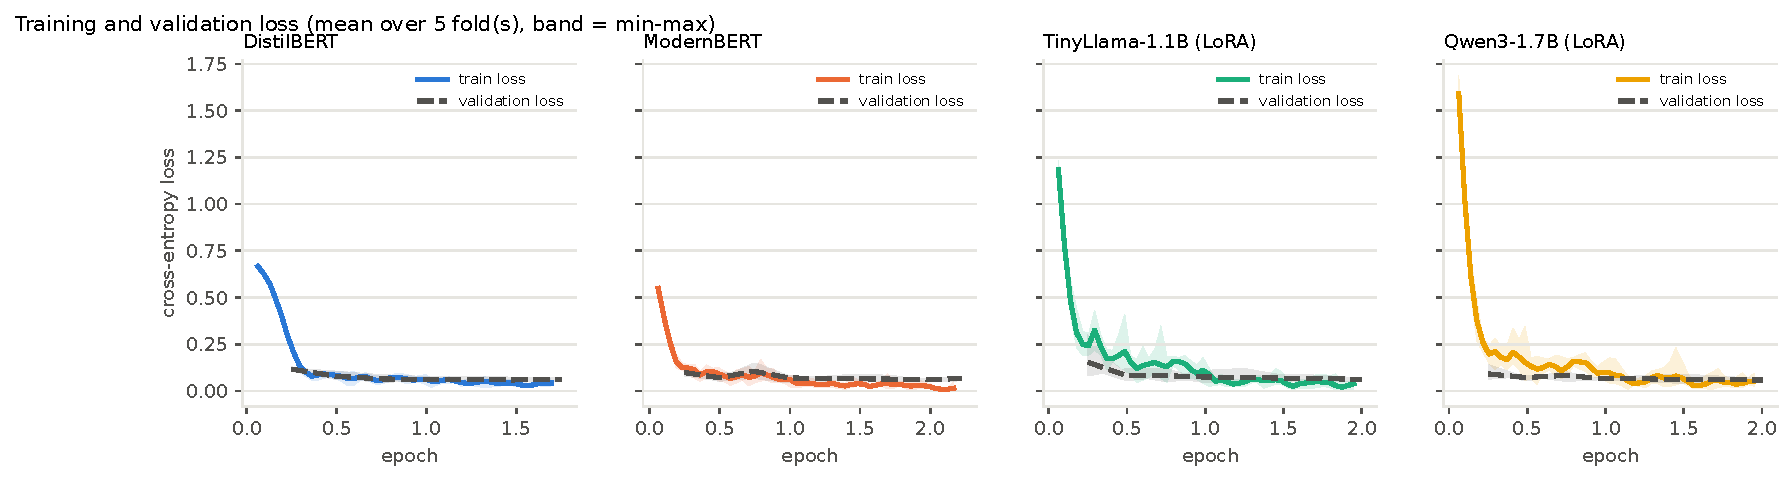
\includegraphics[width=\linewidth]{loss_curves.pdf}
\caption{Training (coloured) and validation (dashed) loss, mean over 5 folds; the band shows the min--max across folds.}
\label{fig:loss}
\end{figure}

\subsection{Behaviour by data source}
\begin{table}[H]
\centering\small
\begin{tabular}{llrrrr}
\toprule
Source & Metric & DistilBERT & ModernBERT & TinyLlama & Qwen3 \\
\midrule
Explicit preference & recall & 0.986 & 0.985 & 0.993 & 0.997 \\
Choice selection (implicit) & recall & 0.999 & 0.998 & 0.999 & 0.997 \\
Persona dialogue turn & recall & 0.970 & 0.973 & 0.975 & 0.980 \\
Persona dialogue turn & false-pos. rate & 0.009 & 0.006 & 0.006 & 0.004 \\
OpenAssistant message & recall & 0.158 & 0.193 & 0.211 & 0.263 \\
OpenAssistant message & false-pos. rate & 0.004 & 0.004 & 0.003 & 0.005 \\
Final question & false-pos. rate & 0.001 & 0.000 & 0.000 & 0.000 \\
Choice initial query & false-pos. rate & 0.000 & 0.000 & 0.000 & 0.000 \\
\bottomrule
\end{tabular}

\caption{Recall on positive rows and false-positive rate on negative rows, by data source (pooled test folds).}
\label{tab:source}
\end{table}

Table~\ref{tab:source} separates the easy from the hard. PrefEval's explicit and choice-based preferences are recalled almost perfectly,
and requests are almost never flagged. Persona turns, where the preference is a passing remark, are found 97--98\% of the time.
The weak spot is \textbf{casual real-chat preferences}: only \pOasstRecLo--\pOasstRecHi\% of the \pOasstPosTest{} OpenAssistant positives
are recalled. Part of this is label noise (those labels were the least reliable in the audit), but the models clearly learned PrefEval's
style of preference better than open-domain chat.

\subsection{Classifier vs.\ a prompted LLM}
\begin{table}[H]
\centering\small
\begin{tabular}{lrrrrr}
\toprule
Detector & F1 & Precision & Recall & Accuracy & ms / message \\
\midrule
DistilBERT & 0.990 & 0.991 & 0.990 & 0.993 & 1.4 \\
ModernBERT & 0.992 & 0.996 & 0.988 & 0.994 & 6.5 \\
TinyLlama-1.1B (LoRA) & 0.993 & 0.993 & 0.992 & 0.995 & 17.1 \\
Qwen3-1.7B (LoRA) & 0.994 & 0.996 & 0.992 & 0.996 & 25.1 \\
Llama-3-8B, zero-shot prompt & 0.879 & 0.787 & 0.996 & 0.896 & 72.0 \\
\bottomrule
\end{tabular}

\caption{The same 2{,}000 PrefEval messages for every detector (out-of-fold predictions for the classifiers). The LLM uses the same
definition, zero-shot.}
\label{tab:llm}
\end{table}

The trained classifiers beat the prompted Llama-3-8B by 11--12 F1 points (Table~\ref{tab:llm}, Figure~\ref{fig:roc}). The LLM catches
nearly every preference (recall \pLlmRec) but also flags about one in six non-preference messages (false-positive rate
\pLlmFpr\%, precision \pLlmPrec), which would fill a
preference memory with noise. DistilBERT is both more accurate (F1 \pDistilSameFOne) and about \pSpeedup$\times$ faster. This supports the proposal's
claim directly. Caveat: some evaluation labels were produced by the same LLM family with different prompts; that shared origin would tend
to favour the LLM, so the gap is if anything conservative.

\begin{figure}[H]
\centering
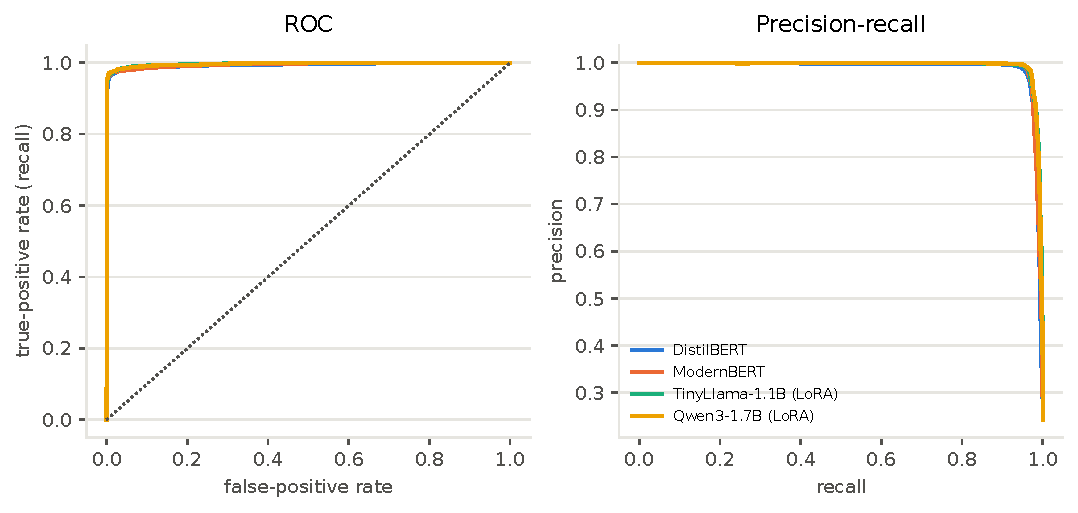
\includegraphics[width=0.85\linewidth]{roc_pr.pdf}
\caption{ROC and precision--recall curves (pooled test folds). The LLM's operating point (\texttimes) lies below every classifier curve.}
\label{fig:roc}
\end{figure}

\subsection{Ensembles}
All 15 non-empty subsets of the four models were combined with three rules: soft voting (mean probability), hard majority vote, and
stacking (logistic regression). Thresholds and stackers are fitted on validation folds only. The best ensemble, \pBestEnsMembers{}, reaches F1
\pBestEnsFOne{}, just $+0.001$ over Qwen3 alone, at about 1.7$\times$ the cost (Table~\ref{tab:ens}). The reason is in the diversity
analysis: the models disagree on at most \pDisagreeMax\% of messages, and their errors are strongly correlated (error correlation
\pErrCorrLo--\pErrCorrHi). They fail on the \emph{same} messages, which are most likely genuinely ambiguous turns or residual label noise,
so combining them cannot recover much.

\begin{table}[H]
\centering\small
\resizebox{\linewidth}{!}{\begin{tabular}{llrrrr}
\toprule
Rule & Members & F1 & Prec. & Rec. & ms (sum) \\
\midrule
Best soft & TinyLlama + Qwen3 & 0.977 & 0.990 & 0.965 & 42.3 \\
Best hard & TinyLlama + Qwen3 & 0.977 & 0.989 & 0.965 & 42.3 \\
Best stacking & DistilBERT + ModernBERT + TinyLlama + Qwen3 & 0.977 & 0.992 & 0.962 & 50.2 \\
\midrule Single & DistilBERT & 0.969 & 0.983 & 0.955 & 1.4 \\
Single & ModernBERT & 0.972 & 0.988 & 0.956 & 6.5 \\
Single & TinyLlama & 0.974 & 0.988 & 0.961 & 17.1 \\
Single & Qwen3 & 0.976 & 0.988 & 0.965 & 25.1 \\
\bottomrule
\end{tabular}
}
\caption{Best ensemble per combination rule vs.\ the single models (pooled test F1; latency summed over members).}
\label{tab:ens}
\end{table}

\begin{figure}[H]
\centering
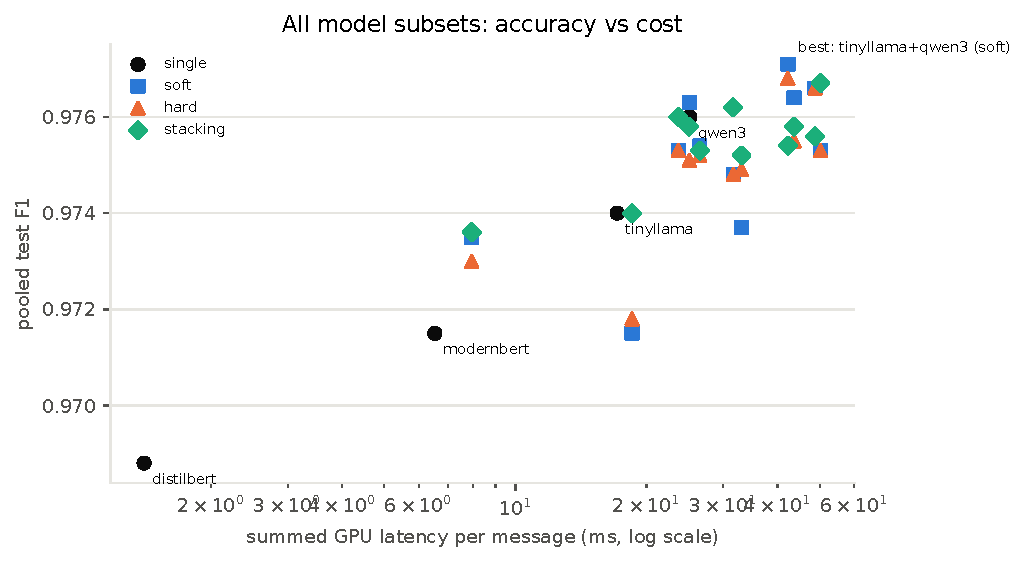
\includegraphics[width=0.62\linewidth]{ensembles.pdf}
\caption{Every subset and rule: F1 vs.\ summed latency (log scale). Ensembles do not move the accuracy--cost frontier.}
\label{fig:ens}
\end{figure}

%===============================================================================
\section{Limitations}
\begin{itemize}
  \item \textbf{Pseudo-labels set a ceiling on measurement.} About 70\% of rows carry refined LLM labels with roughly 90\% audited agreement.
        On those rows, test scores partly measure agreement with the labeller. Scores on gold rows (explicit, choice, questions) are the most
        trustworthy.
  \item \textbf{The refinement rules were designed after seeing the audit}, and the ``after'' agreement is measured on the same 200 rows.
        A fresh audit sample would give an unbiased estimate.
  \item \textbf{Real-chat recall is low} (\pOasstRecLo--\pOasstRecHi\%). This matters little for Phase~3, which is evaluated on PrefEval, but it
        limits claims about open-domain preference detection.
  \item \textbf{One seed per fold.} Fold-to-fold variation (std 0.004--0.007) is reported; repeated seeds were not run.
\end{itemize}

%===============================================================================
\section{Implications for Phase 3}
\begin{itemize}
  \item \textbf{Detector:} DistilBERT as the default (F1 0.969, \pDistilLat\,ms per message, 0.4\% false alarms on real chat); Qwen3 as the
        maximum-accuracy variant. Ensembling is not worth its cost.
  \item \textbf{Leakage-free use:} each fold's model is applied only to that fold's held-out topics, which covers all 20 topics in Phase~3
        without any topic seen in training.
  \item \textbf{Memory quality:} near-zero false alarms on LMSYS turns mean the distractor turns Phase~3 replays will not pollute the memory.
\end{itemize}

%===============================================================================
\section{Conclusion}
Phase~2 delivers a reproducible preference-detection pipeline. It covers turn-level data with audited and refined pseudo-labels, leakage-controlled
topic cross-validation, four classifiers, all their ensembles, and a direct comparison with LLM prompting. A 66M-parameter DistilBERT
detects preferences on unseen topics with F1 0.969, beats a prompted 8B LLM by more than 10 F1 points on the same data, and runs about
\pSpeedup$\times$ faster. That is the component Phase~3 needs.

\begin{thebibliography}{9}\small
\bibitem{prefeval} S.~Zhao et al. \emph{Do LLMs Recognize Your Preferences? Evaluating Personalized Preference Following in LLMs.} ICLR 2025.
\bibitem{distilbert} V.~Sanh et al. \emph{DistilBERT, a distilled version of BERT.} arXiv:1910.01108, 2019.
\bibitem{modernbert} B.~Warner et al. \emph{Smarter, Better, Faster, Longer: A Modern Bidirectional Encoder (ModernBERT).} arXiv:2412.13663, 2024.
\bibitem{tinyllama} P.~Zhang et al. \emph{TinyLlama: An Open-Source Small Language Model.} arXiv:2401.02385, 2024.
\bibitem{qwen3} Qwen Team. \emph{Qwen3 Technical Report.} arXiv:2505.09388, 2025.
\bibitem{lora} E.~Hu et al. \emph{LoRA: Low-Rank Adaptation of Large Language Models.} ICLR 2022.
\bibitem{oasst} A.~K\"opf et al. \emph{OpenAssistant Conversations.} NeurIPS 2023 Datasets and Benchmarks.
\end{thebibliography}

\appendix
\section{Reproducing the results}
Branch \nolinkurl{phase2-classifier}; documentation in \nolinkurl{docs/PHASE2.md}; configs in \nolinkurl{configs/phase2/}.
\begin{verbatim}
conda create -n prefeval-p2 python=3.11 && conda activate prefeval-p2
pip install -r requirements-phase2.txt
# stages in order: data, pseudo, splits, train, baseline, analyze
python -m phase2.pipeline --stage data
python report/make_assets_phase2.py   # this report's numbers
\end{verbatim}
Every number in this report is generated from \nolinkurl{data/phase2/} and \nolinkurl{results/phase2/} by that script.

\section{Use of AI assistance}
Claude (Anthropic) was used as a coding and writing assistant for the pipeline, the analysis and the drafting of this report. The audit labels
were assigned by me; all experiments ran on my machine, and every reported number is produced by scripts from the logged results.

\end{document}
